\documentclass[]{article}
\usepackage{lmodern}
\usepackage{amssymb,amsmath}
\usepackage{ifxetex,ifluatex}
\usepackage{fixltx2e} % provides \textsubscript
\ifnum 0\ifxetex 1\fi\ifluatex 1\fi=0 % if pdftex
  \usepackage[T1]{fontenc}
  \usepackage[utf8]{inputenc}
\else % if luatex or xelatex
  \ifxetex
    \usepackage{mathspec}
  \else
    \usepackage{fontspec}
  \fi
  \defaultfontfeatures{Ligatures=TeX,Scale=MatchLowercase}
\fi
% use upquote if available, for straight quotes in verbatim environments
\IfFileExists{upquote.sty}{\usepackage{upquote}}{}
% use microtype if available
\IfFileExists{microtype.sty}{%
\usepackage{microtype}
\UseMicrotypeSet[protrusion]{basicmath} % disable protrusion for tt fonts
}{}
\usepackage[margin=1in]{geometry}
\usepackage{hyperref}
\hypersetup{unicode=true,
            pdftitle={Variants of Populism},
            pdfborder={0 0 0},
            breaklinks=true}
\urlstyle{same}  % don't use monospace font for urls
\usepackage{graphicx,grffile}
\makeatletter
\def\maxwidth{\ifdim\Gin@nat@width>\linewidth\linewidth\else\Gin@nat@width\fi}
\def\maxheight{\ifdim\Gin@nat@height>\textheight\textheight\else\Gin@nat@height\fi}
\makeatother
% Scale images if necessary, so that they will not overflow the page
% margins by default, and it is still possible to overwrite the defaults
% using explicit options in \includegraphics[width, height, ...]{}
\setkeys{Gin}{width=\maxwidth,height=\maxheight,keepaspectratio}
\IfFileExists{parskip.sty}{%
\usepackage{parskip}
}{% else
\setlength{\parindent}{0pt}
\setlength{\parskip}{6pt plus 2pt minus 1pt}
}
\setlength{\emergencystretch}{3em}  % prevent overfull lines
\providecommand{\tightlist}{%
  \setlength{\itemsep}{0pt}\setlength{\parskip}{0pt}}
\setcounter{secnumdepth}{0}
% Redefines (sub)paragraphs to behave more like sections
\ifx\paragraph\undefined\else
\let\oldparagraph\paragraph
\renewcommand{\paragraph}[1]{\oldparagraph{#1}\mbox{}}
\fi
\ifx\subparagraph\undefined\else
\let\oldsubparagraph\subparagraph
\renewcommand{\subparagraph}[1]{\oldsubparagraph{#1}\mbox{}}
\fi

%%% Use protect on footnotes to avoid problems with footnotes in titles
\let\rmarkdownfootnote\footnote%
\def\footnote{\protect\rmarkdownfootnote}

%%% Change title format to be more compact
\usepackage{titling}

% Create subtitle command for use in maketitle
\newcommand{\subtitle}[1]{
  \posttitle{
    \begin{center}\large#1\end{center}
    }
}

\setlength{\droptitle}{-2em}
  \title{Variants of Populism}
  \pretitle{\vspace{\droptitle}\centering\huge}
  \posttitle{\par}
\subtitle{A Cross-National Examination of Support for European Populist Parties}
  \author{}
  \preauthor{}\postauthor{}
  \date{}
  \predate{}\postdate{}

\usepackage{microtype}
\usepackage{lmodern}
\usepackage{enumitem}
\usepackage[ngerman, english]{babel}

\begin{document}
\maketitle

\begin{center}

\textbf{Fabio Votta}, \textit{B.A. University of Stuttgart.} Contact: \href{fabio.votta@gmail.com}{fabio.votta@gmail.com}

\textbf{Nga Nguyen}, \textit{B.A. Institut d'Etudes Politiques de Bordeaux.} Contact: \href{nga.nguyen@scpobx.fr}{nga.nguyen@scpobx.fr}

\textbf{Marlon Schumacher}, \textit{B.A. University of Stuttgart.} Contact: \href{m.c.schumacher@live.de}{m.c.schumacher@live.de}

\end{center}

\vspace{0.5cm}

\pagenumbering{gobble}

This paper seeks to investigate support for populist parties in Europe.
While populism is an intensely debated topic, most scholarship is
plagued with conceptual conflations between different variants of
populism.

To avoid such conceptual confusions, this paper adopts a minimalist
definition to identify core features that all subtypes of populism have
in common, namely anti-establishment attitudes as well as their
opposition to globalization.

While previous authors used economic and cultural factors to determine
support for populism, we propose a theoretical model that distinguishes
between \emph{traditionalist} and \emph{progressive populism}. This
model involves two steps:

\begin{enumerate}
\renewcommand{\labelenumii}{\alph{enumii}.}
\item \textbf{Economically deprived individuals} are more likely to reject establishment parties and consequently support populist parties instead. 
\item \textbf{Cultural values} determine whether these individuals support progressive or traditionalist populism: 
\begin{enumerate}
\item \textit{Traditionalist populists} draw their support from people who believe  that societal change has gone too far.
\item \textit{Progressive populists} draw their support from people who believe that their reactionary society is in need of progressive change.
\end{enumerate}
\end{enumerate}

In order to operationalize our conceptual considerations, we use the
\emph{Chapel Hill Expert Survey} dataset and combine it with
\emph{European Social Survey} data to identify respondents that vote for
and/or identify with populist parties.

We estimate a multinomial logistic regression to test our hypotheses.
Our models lend support for our theoretical expectations. Economically
deprived individuals are more likely to support either variant of
populism. Yet individuals who hold traditional values are more likely to
support traditionalist populism, whereas the effect goes in the opposite
direction for the support of progressive populism.

Further research might be able to build upon our conceptualization and
give more attention to the different variants of populism, so as to not
conflate the distinct explanatory frameworks that come along with them.

\newpage

\begin{center}
{\LARGE \textbf{Preliminary Results}}
\end{center}

\vspace{0.2cm}

\begin{center}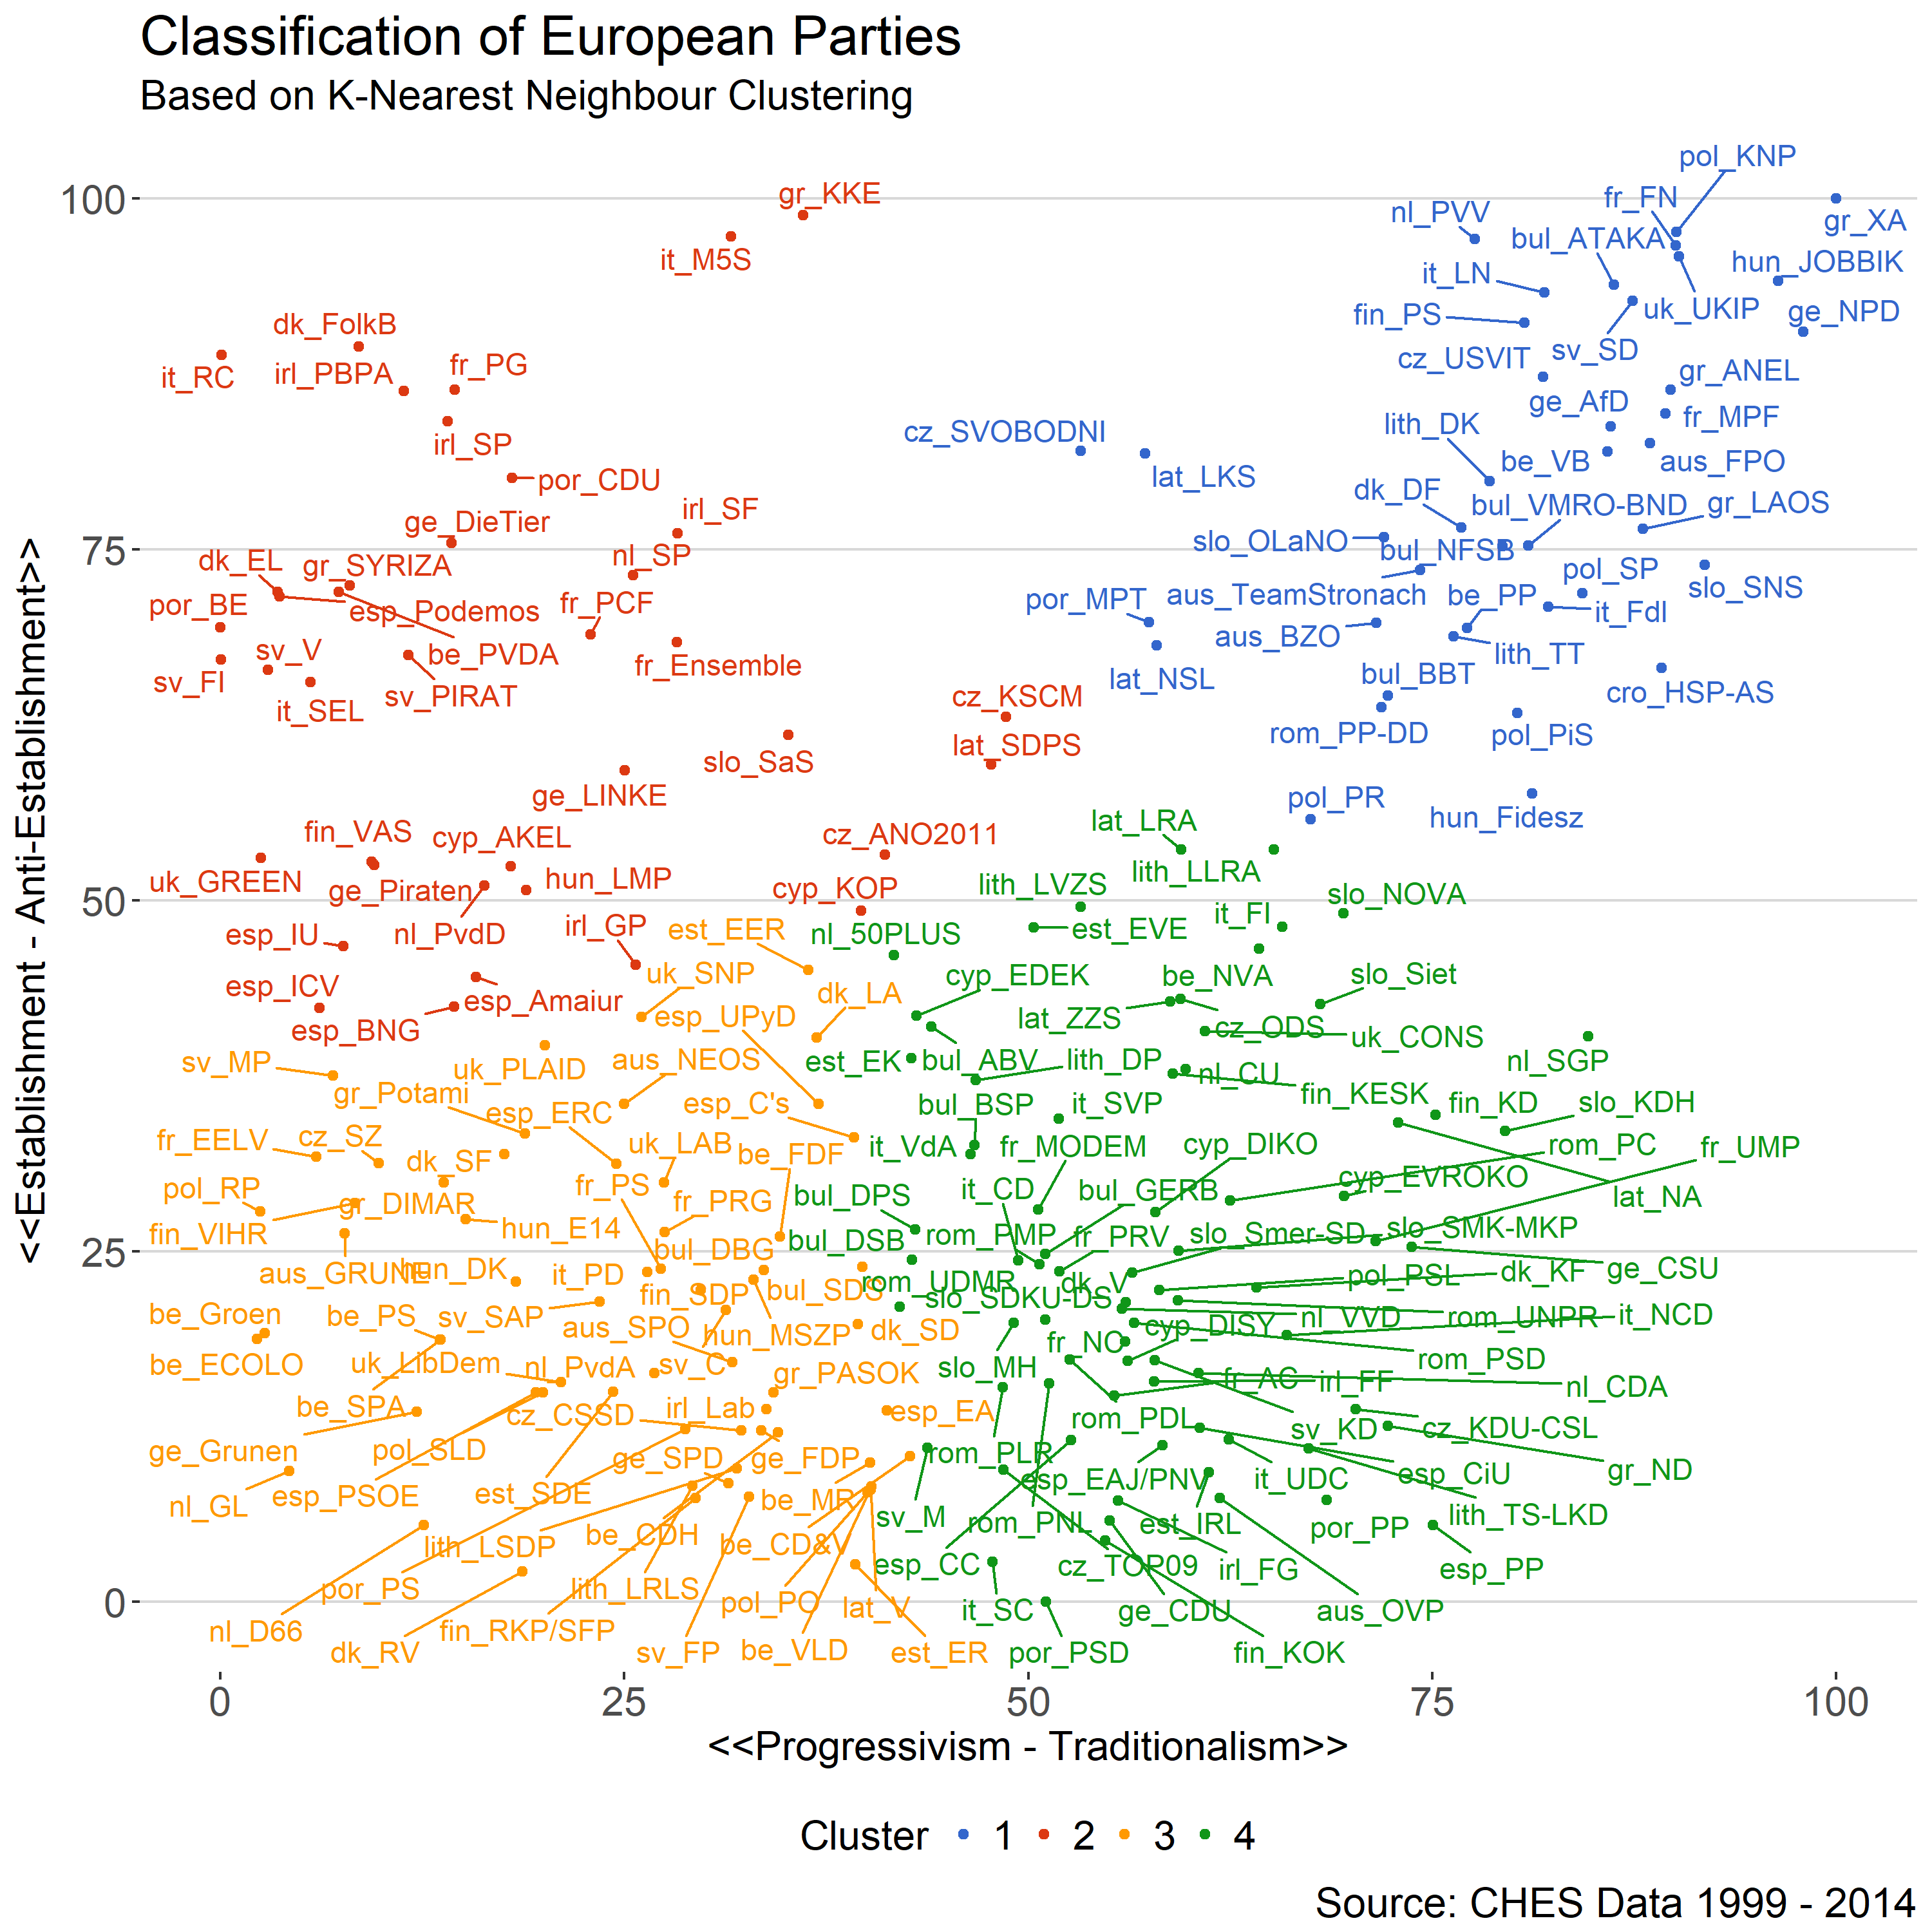
\includegraphics[height=0.55\textheight]{images/party_alignment_abstract} \end{center}

\vspace{1cm}

\begin{center}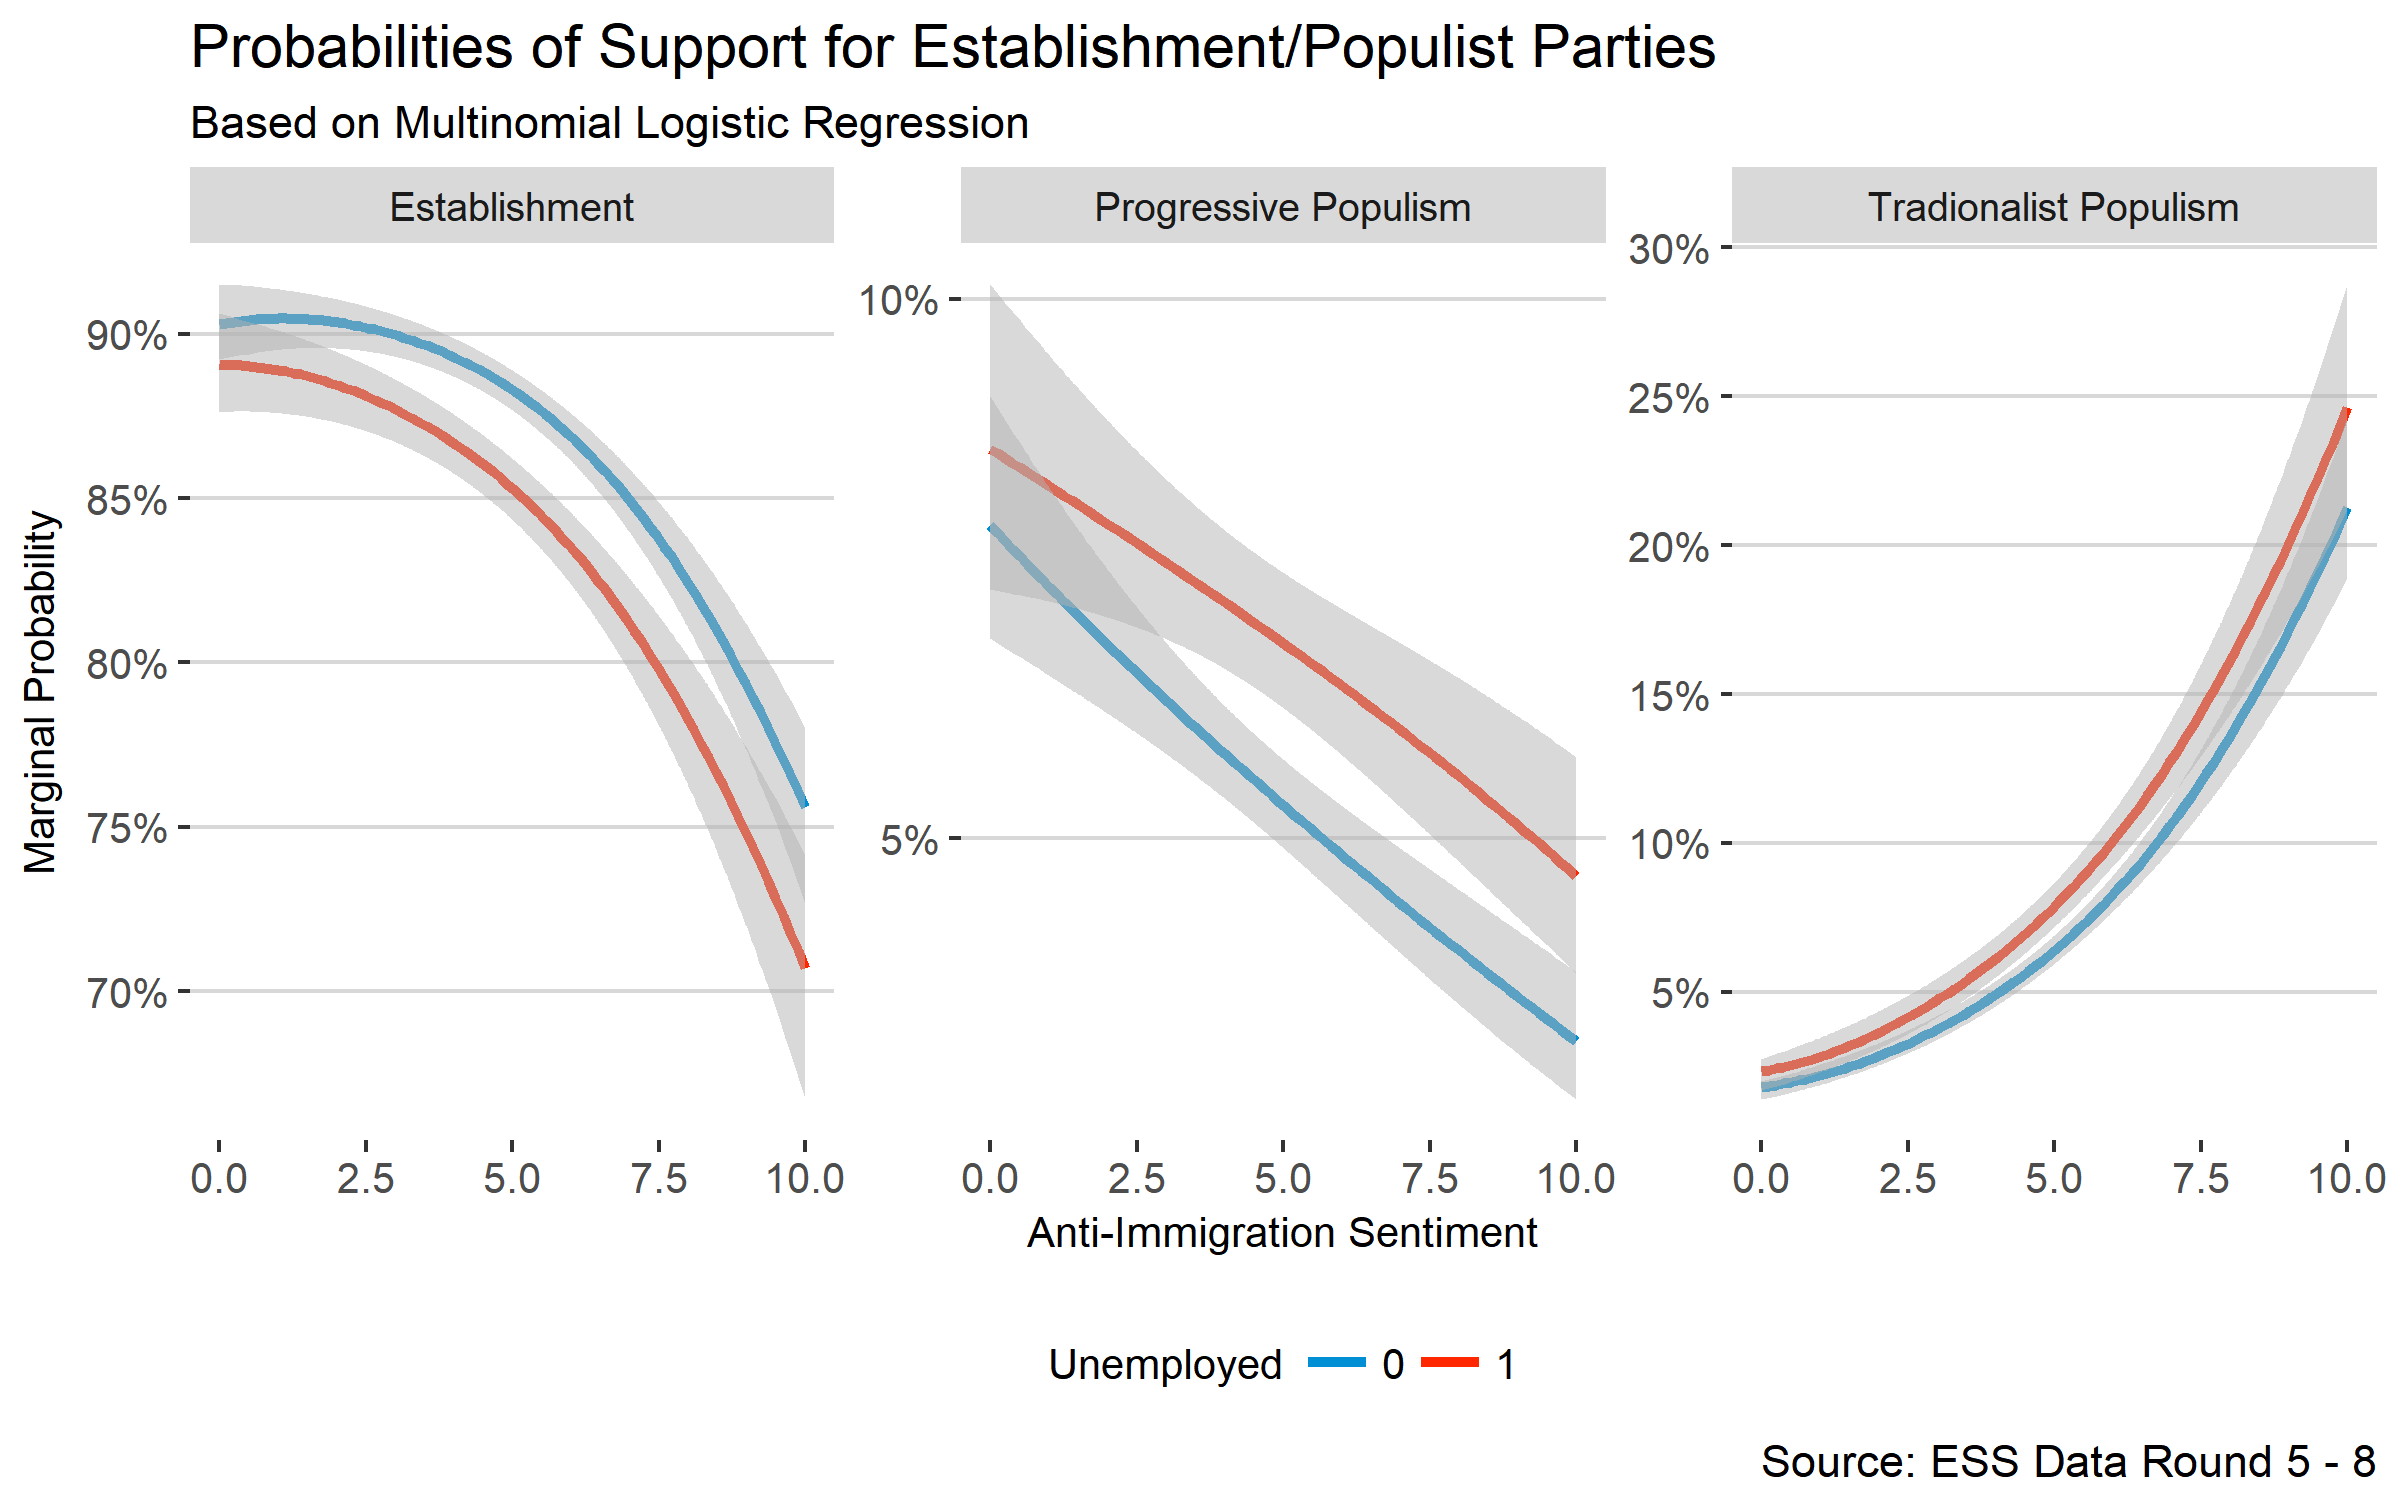
\includegraphics[height=0.35\textheight]{images/interaction_abstract} \end{center}


\end{document}
